\section{Path integrals}
\label{A:autoparam path_integrals}

Making use of the fact
\[
dt = -\frac{du}{uv},
\]
we change the time integrals
\[
{T_{i}(z)}\equiv\int_0^{\period_{i}} dt, \qquad \INT_{i}^{j}\equiv\int_0^{\period_{i}} \frac{1}{u_1^j(t)}dt
\] 
to path integrals with respect to the fast variable $u_1(t),u_2(t)$. This process effectively removes the fast variable $u_1(t),u_2(t)$. To this end, for an arbitrary value of $h$ we define from~\eqref{E:AvgH}
\begin{equation}
u_2^{\pm}= \pm \sqrt{\frac{I u_1 - u_1^3 - 2 h}{u_1}} \equiv \pm\sqrt{f(u_1)}
\end{equation}
and the intersections of the periodic orbits with the $u_1$-axis are obtained by solving
\begin{equation}\label{E:roots}
\begin{aligned} 
I u_1 - u_1^3 - 2 h = (u_1^- - u_1)(u_1^+ - u_1)(u_1^* - u_1) = 0\\
u_1^- u_1^+ u_1^* = - 2 h, \quad u_1^- u_1^+ + u_1^- u_1^* + u_1^+ u_1^* = -I,\quad u_1^- + u_1^+ + u_1^* = 0
\end{aligned}
\end{equation}
where two of the three roots $\bar{u}_1^{-},\;\bar{u}_1^{+}$ represent the intersections of an orbit of energy level $H$ encircling the elliptic fixed point, while the third root $\bar{u}_1^{*}$ corresponds to the intersection of the orbit which lies out side the heteroclinic orbit but of the same energy level $H$. It is clear that at the elliptic fixed point $B^+$, $H$ is positive and since the fixed point lies on the right hand plane, the intersections $u_1^{-}$ and $u_1^{+}$ (points where the periodic orbit intersects the $u_1-$axis, i.e., the points where $u_2 = 0$) are positive while $u_1^{*}$ is negative, i.e,
\[
0 \leqslant h \leqslant \frac{I}{3}\sqrt{\frac{I}{3}}, \qquad u_1^{{2}^{*}} \leqslant
\, 0 \, \leqslant u_1^{2^-} \leqslant u_1^{2^+}.
\]
Similarly for the elliptic fixed point $B^-$, $H$ is negative and it can be shown that $u_1^-$ and $u_1^+$ are negative while $u_1^{*}$ is positive, i.e.,
\[
-\frac{I}{3}\sqrt{\frac{I}{3}} \leqslant h \leqslant 0, \qquad u_1^{{1}^{-}} \le
u_1^{{1}^{+}} \leqslant \, 0 \, \leqslant u_1^{{1}^{*}}.
\]
Due to the symmetry of the phase plane, we have
\begin{equation}
\begin{aligned} 
\lambda_1=u_1^{{2}^{+}}=-u_1^{{1}^{-}},\qquad \lambda_2=u_1^{{2}^{-}}=-u_1^{{1}^{+}},\qquad \lambda_3=u_1^{{2}^{*}}=-u_1^{{1}^{*}}
\end{aligned}\label{E:intersects}
\end{equation}
where superscript $1$ represents the region $u_1<0, H<0$ while superscript $2$ represents the region $u_1>0, H>0$. A sample plot of the three roots is shown in Figure~\ref{F:lambdas}.
\begin{figure}
\begin{center}
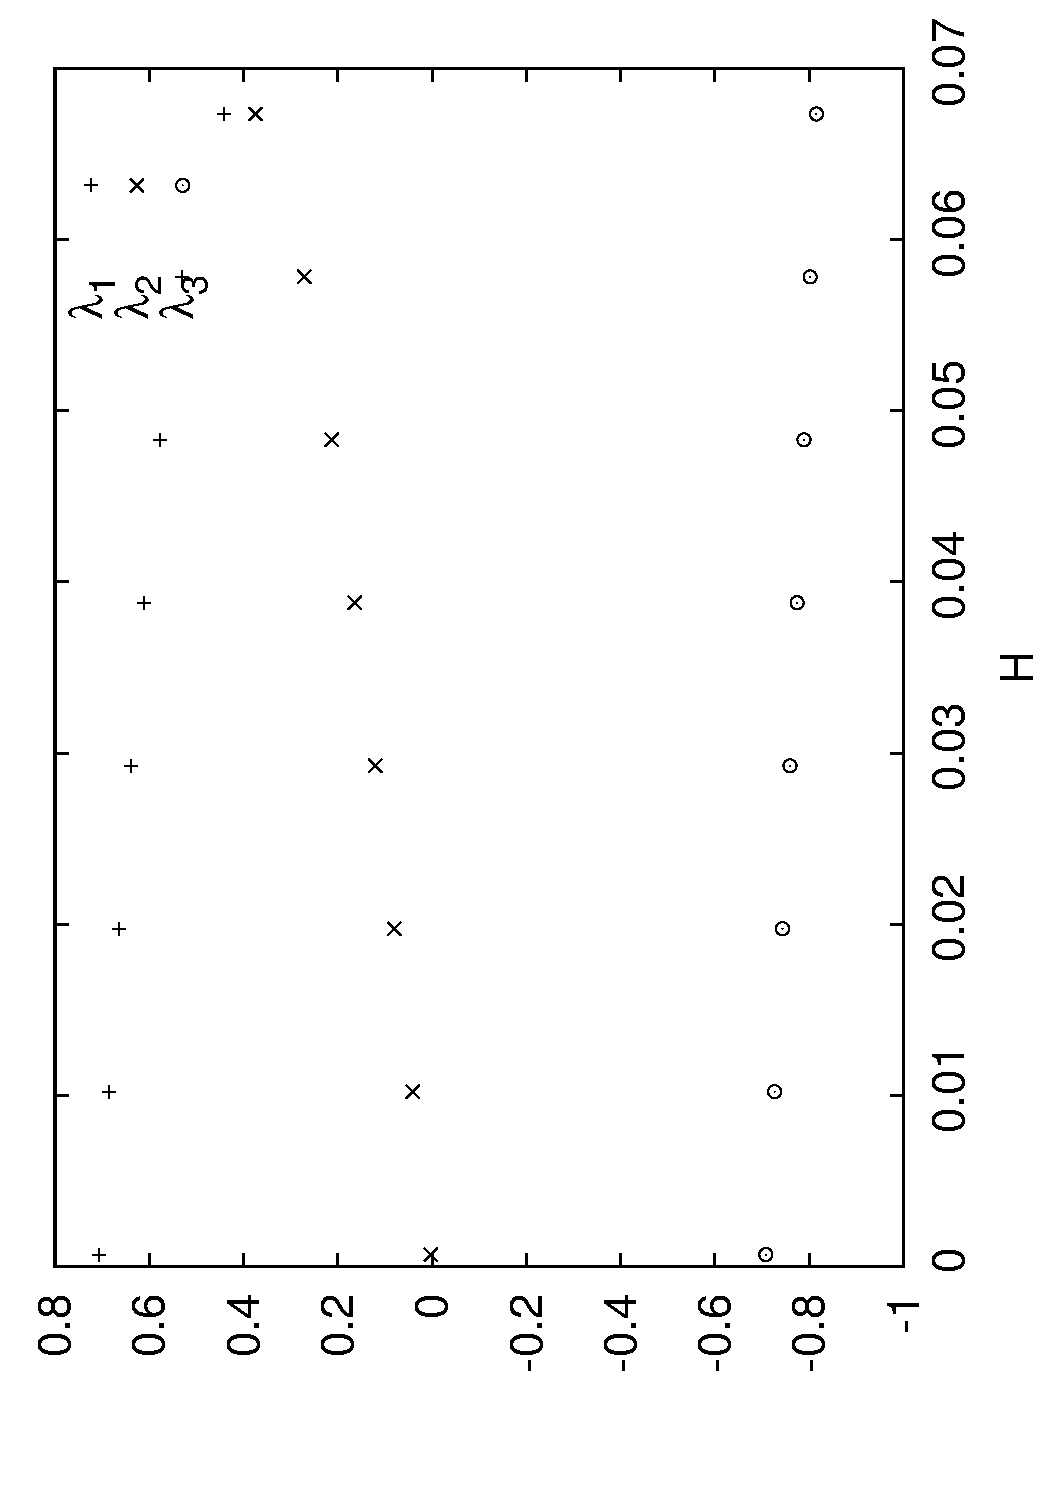
\includegraphics[angle=-90,width=\textwidth*7/8]{figures/lambdas}
\caption{Three roots shown for $I = 0.5$ and $0\le h \le H_c$. This figure is meant to help understand the limiting value of $\kappa$ which in turns helps in evaluating the gluing boundary condition}
\label{F:lambdas}
\end{center}
\end{figure}
Since the roots of $I u_1 - u_1^3 + 2 h$ for $h \le 0$ are the same as the roots of $I u_1 - u_1^3 - 2 h$ for $h \ge 0$, keeping the order $u_1^{2^+} > u_1^{2^-} > 0 > u_1^{2^*}$
\[
\begin{aligned}
\period_1(z)= \period_2(z) &= 2\int_{u_1^{{2}^{-}}}^{u_1^{{2}^{+}}}\frac{dt}{\sqrt{ t \,(I t - t^3 - 2 h)}}=2\, g K(\kappa)
\end{aligned}
\]
where
\[
g \equiv \frac{2}{\sqrt{\lambda_1 (\lambda_2-\lambda_3)}}, \qquad
\kappa^2 \equiv \frac{\lambda_3(\lambda_2 - \lambda_1)}{\lambda_1
(\lambda_2 - \lambda_3)} >0 ,\qquad \kappa^2 < \alpha^2 \equiv
\frac{\lambda_1 - \lambda_2}{\lambda_1} < 1
\]
By \citet[formula 256.12]{byrd54:_handb_of_ellip_integ_for}, the integrals
$\INT_{j}^1$,
% \[
% \begin{aligned}
%  \INT_1^1&\equiv\int_0^{\period_1}\frac{dt}{u_1(t)} = -
%
%
%  2\int_{u_1^{{1}^{-}}}^{u_1^{{1}^{+}}}\frac{d %u_1}{u_1^2\,\sqrt{f(u_1)}} \quad \text{for} \quad u_1 \le 0,\; h<0\\
%   \INT_2^1&\equiv\int_0^{\period_2}\frac{dt}{u_1(t)} =
%
%
%   2\int_{u_1^{{2}^{-}}}^{u_1^{{2}^{+}}}\frac{d %u_1}{u_1^2\,\sqrt{f(u_1)}} \quad \text{for} \quad u_1 \ge 0,\; h>0
%   \end{aligned}
% \]
reduce to
\begin{align*}
-\INT_1^1 = \INT_2^1 &= 2\int_{u_1^{2^-}}^{u_1^{2^+}} \frac{dt}{t \sqrt{t (I t - t^3 - 2 h)}}\\
&= 2 \int_{u_1^{2^-}}^{u_1^{2^+}} \frac{dt}{t \sqrt{t (u_1^{2^+}-t)(t-u_1^{2^-})(t-u_1^{2^*})}} = A_1 K(\kappa) + B_1 E(\kappa),
\end{align*}
where
\[
\begin{aligned}
 A_1&=2\,{\frac {g\left(\kappa-\alpha\right)\left
    (\kappa+\alpha\right)}{ \lambda_2{\kappa}^2}}= {\frac
  {4}{\lambda_3 \sqrt {\lambda_1 \left(\lambda_2 - \lambda_3
    \right)}\;}}\\
 B_1 &=2\,{\frac {g{\alpha}^2}{\lambda_2{\kappa}^2}}=
 \frac{4(\lambda_3 - \lambda_2)}{\lambda_2 \lambda_3 \sqrt
  {\lambda_1\left( \lambda_2-\lambda_3\right)}}
\end{aligned}
\]
Similarly, we can show the second set of integrals $\INT_{j}^2$
reduces to
\[
\begin{aligned}
 \INT_1^2 = \INT_2^2 &=
 2\int_{u_1^{{2}^{-}}}^{u_1^{{2}^{+}}}\frac{dt}{t^2\,\sqrt{ t \,(I t - t^3 - 2 h)}}\\
 &=2 \int_{u_1^{{2}^{-}}}^{u_1^{{2}^{+}}}\frac{dt}{t^2\,\sqrt{ t
   \, (u_1^{{2}^{+}}-t)(t-u_1^{{2}^{-}})(t-u_1^{{2}^{*}})}} =
 A_2\, K(\kappa) + B_2\, E(\kappa)
\end{aligned}
\]
where
\[
\begin{aligned}
 A_2&= \frac{2}{3}\,{\frac {g\left
    (3\,{\kappa}^4-6\,{\alpha}^2{\kappa}^2+2\,{
     \alpha}^4+{\alpha}^4{\kappa}^2\right
   )}{{\lambda_2}^2{\kappa}^4}}\\
 &= \frac{4}{3}\,{\frac {\left
    ({\lambda_3}^2+{\lambda_2}^2-2\,\lambda
    _3\lambda_2\right){\kappa}^2}{\sqrt
   {\lambda_1\left( \lambda_2-\lambda_3\right
    )}{\lambda_2}^2{\lambda_3}
   ^2}}+\frac{4}{3}\,{\frac
  {-{\lambda_3}^2+2\,\lambda_3\lambda_2
   +2\,{\lambda_2}^2}{\sqrt {\lambda_1\left
     (\lambda_2-
     \lambda_3\right)}{\lambda_2}^2{\lambda_3}^2}}\\
B_2 &=-\frac{4}{3}\,{\frac {g{\alpha}^2\left(-3\,{\kappa}^2+{\alpha}^2+{
\alpha}^2{\kappa}^2\right)}{{\lambda_2}^2{\kappa}^{4}}}\\
& = -\frac{8}{3} {\frac{\left(\lambda_2-\lambda_3\right)^2{\kappa}^{2}}{\sqrt{\lambda_1\left(\lambda_2-\lambda_3\right)}{\lambda_2}^2{\lambda_3}^2}}-\frac{8}{3}\,{\frac{\left(\lambda_2-\lambda_3\right)\left(\lambda_2+2\,\lambda_3\right)}{\sqrt{\lambda_1\left(\lambda_2-\lambda_3\right)}{\lambda_2}^2{\lambda_3}^2}}
\end{aligned}
\]

The drift and diffusion terms are evaluated making use of these
results.
